\documentclass[beamer]{standalone}

\begin{document}
	\begin{frame}
		\color{blue}\centering\Huge{\textbf{Accelerazione}}	
	\end{frame}
	
	\begin{frame}{{Accelerazione}}
		\centering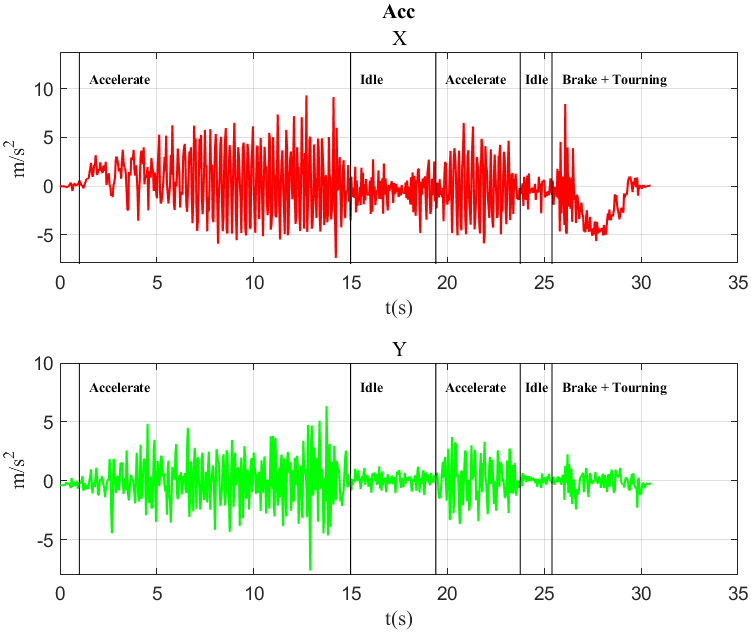
\includegraphics[height=.8\textheight]{figure/Acc/Acc}
	\end{frame}
	
	\begin{frame}{{Media}}
		\centering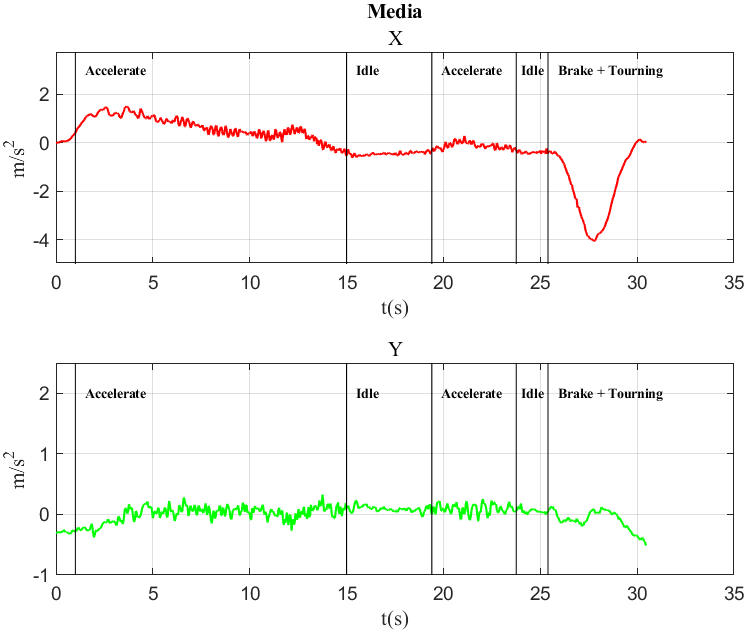
\includegraphics[height=.8\textheight]{figure/Acc/Media}
	\end{frame}
	
	\begin{frame}{{Media Rettificata}}
		\centering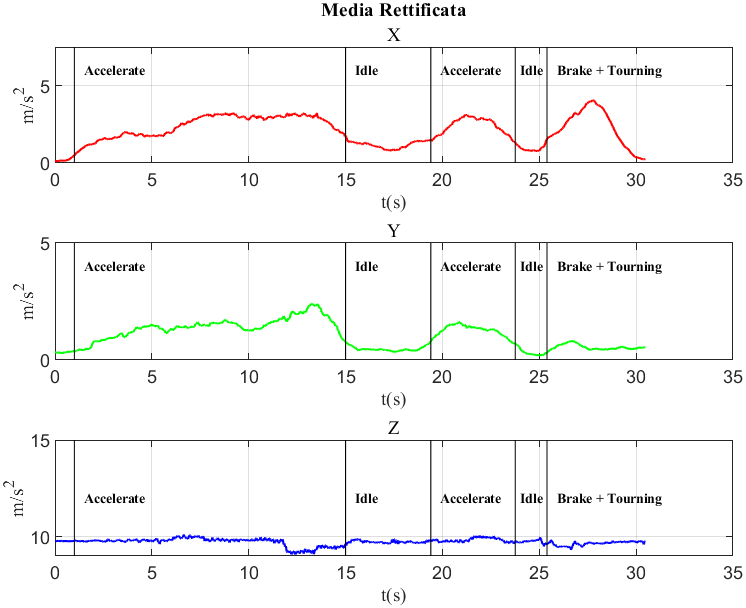
\includegraphics[height=.8\textheight]{figure/Acc/Media Rettificata}
	\end{frame}

	\begin{frame}{{Varianza}}
		\centering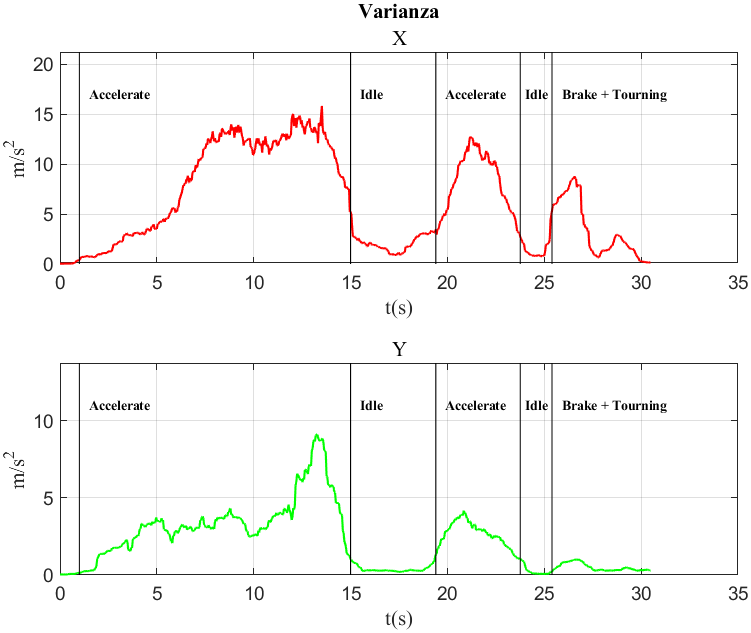
\includegraphics[height=.8\textheight]{figure/Acc/Varianza}
	\end{frame}
	
	\begin{frame}{{Deviazione Standard}}
		\centering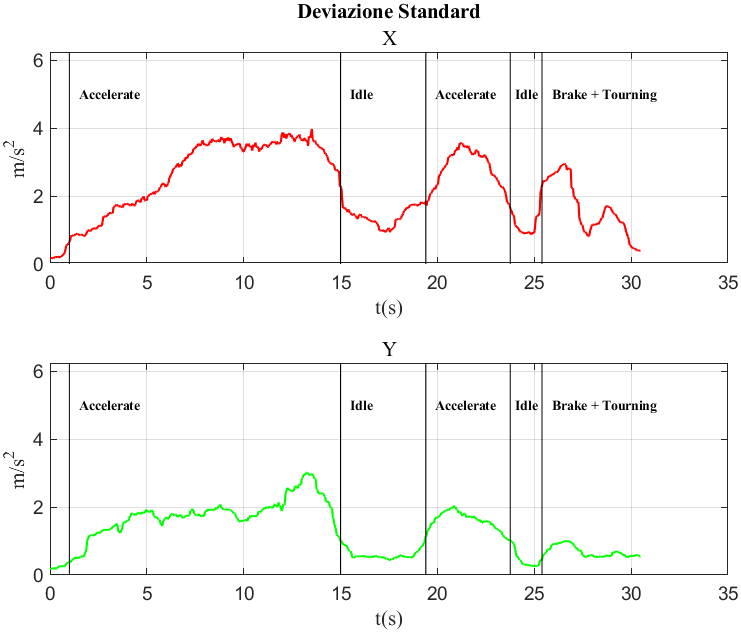
\includegraphics[height=.8\textheight]{figure/Acc/Deviazione Standard}
	\end{frame}
	
	\begin{frame}{{Scarto Quadratico Medio}}
		\centering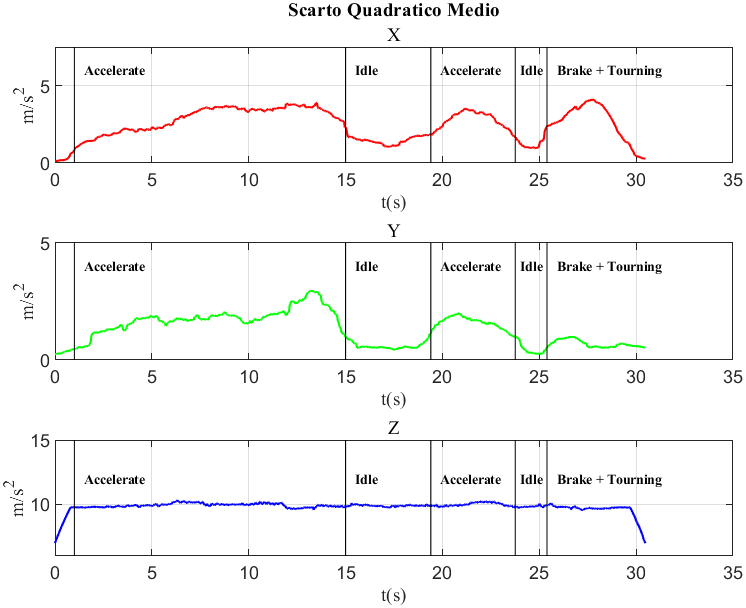
\includegraphics[height=.8\textheight]{figure/Acc/Scarto Quadratico Medio}
	\end{frame}
	
	\begin{frame}{{Max}}
		\centering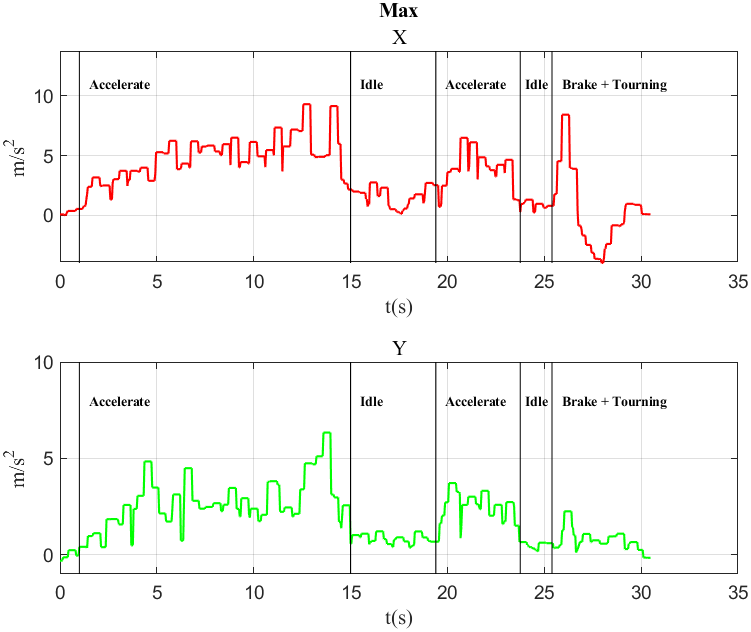
\includegraphics[height=.8\textheight]{figure/Acc/Max}
	\end{frame}
	
	\begin{frame}{{Min}}
		\centering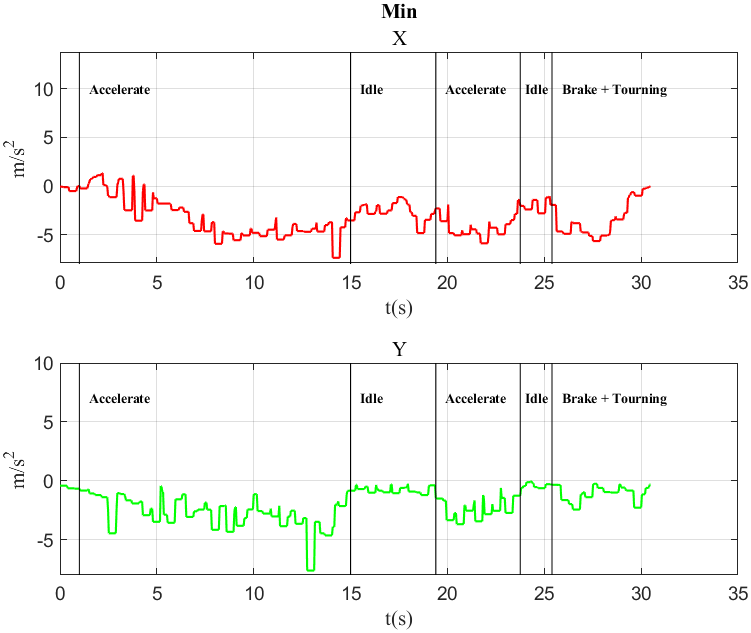
\includegraphics[height=.8\textheight]{figure/Acc/Min}
	\end{frame}

	\begin{frame}{{Peak}}
		\centering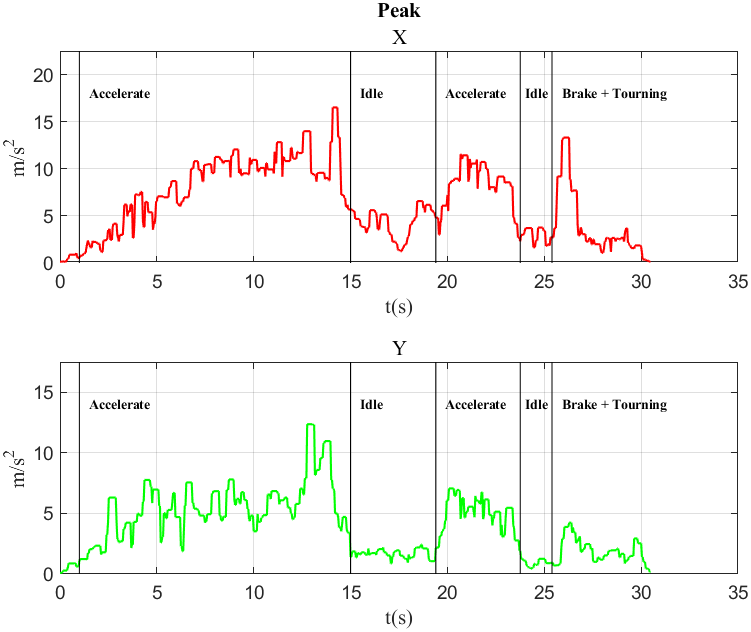
\includegraphics[height=.8\textheight]{figure/Acc/Peak}
	\end{frame}
	
	\begin{frame}{{Kurtosi}}
		\centering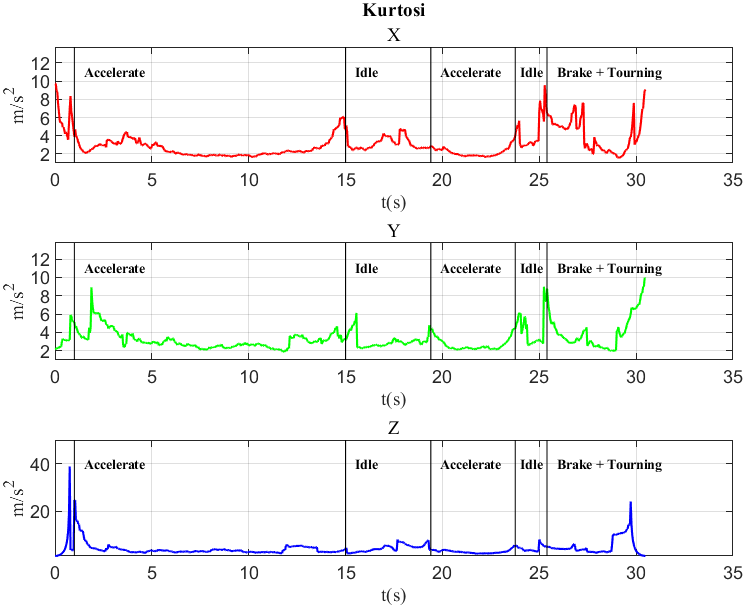
\includegraphics[height=.8\textheight]{figure/Acc/Kurtosi}
	\end{frame}
	
	\begin{frame}{{Skewness}}
		\centering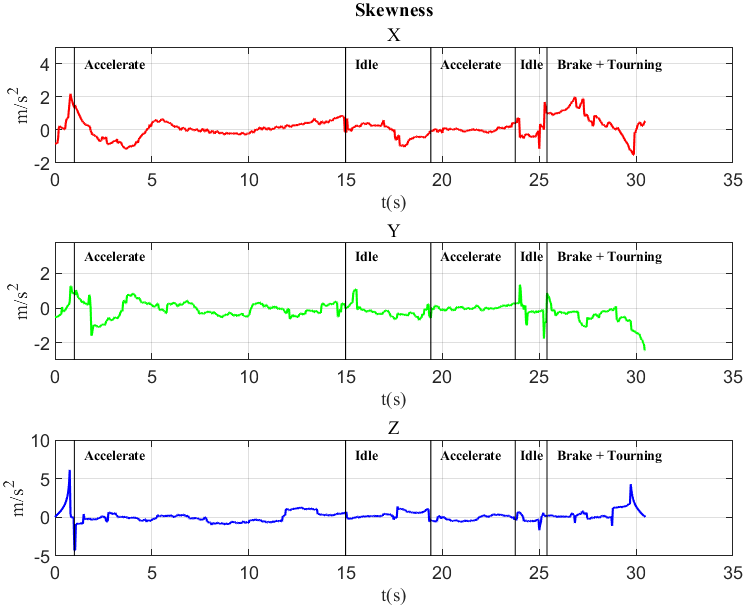
\includegraphics[height=.8\textheight]{figure/Acc/Skewness}
	\end{frame}
	
	\begin{frame}{{Shape Factor}}
		\centering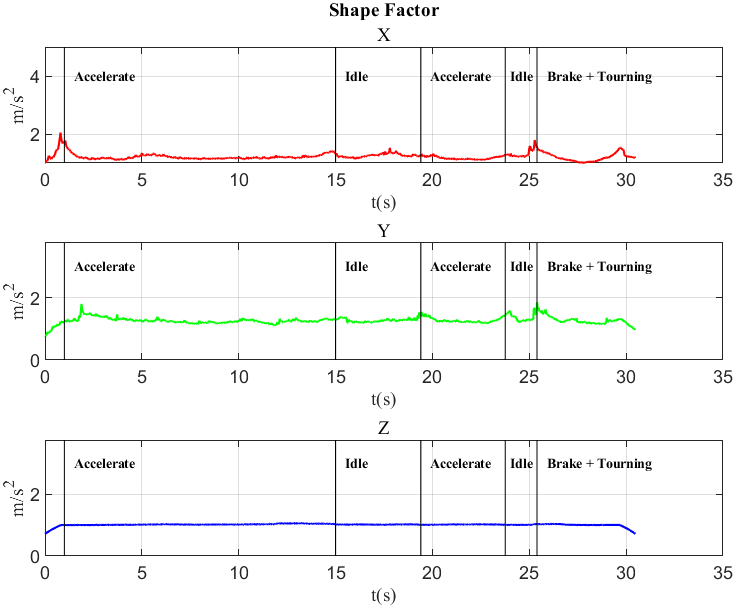
\includegraphics[height=.8\textheight]{figure/Acc/Shape Factor}
	\end{frame}
	
	\begin{frame}{{Crest Factor}}
		\centering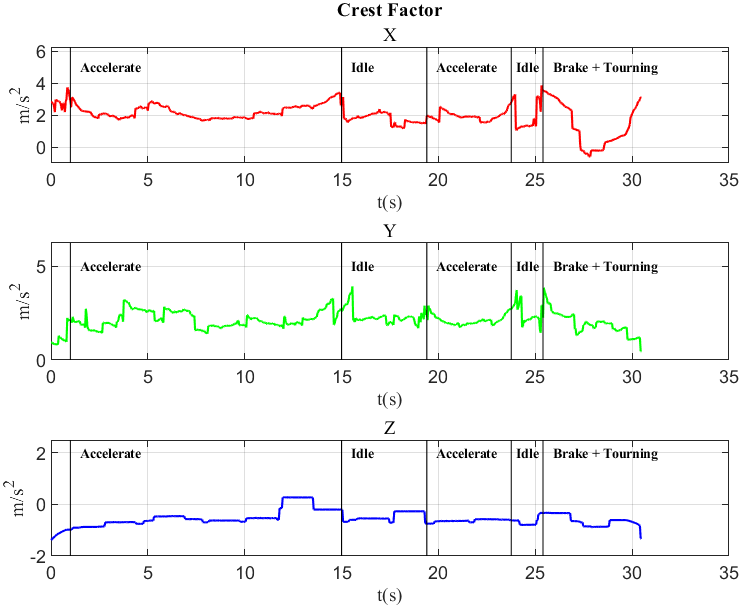
\includegraphics[height=.8\textheight]{figure/Acc/Crest Factor}
	\end{frame}
	
	\begin{frame}{{Impulse Factor}}
		\centering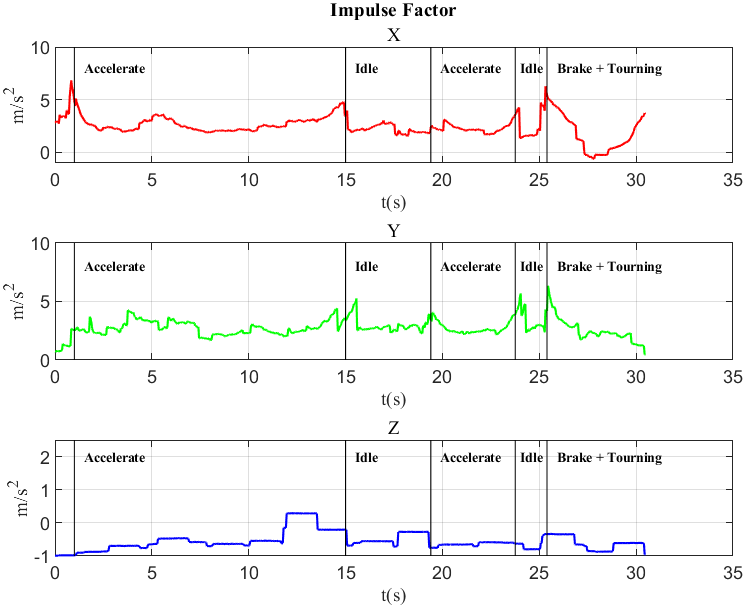
\includegraphics[height=.8\textheight]{figure/Acc/Impulse Factor}
	\end{frame}
	
	\begin{frame}{{Margin Factor}}
		\centering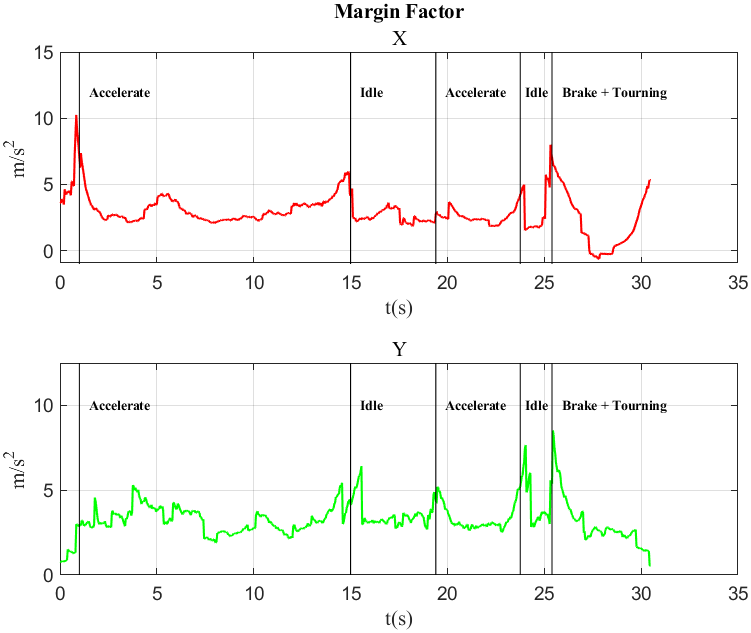
\includegraphics[height=.8\textheight]{figure/Acc/Margin Factor}
	\end{frame}
	
	\begin{frame}{{Trasformata}}
		\centering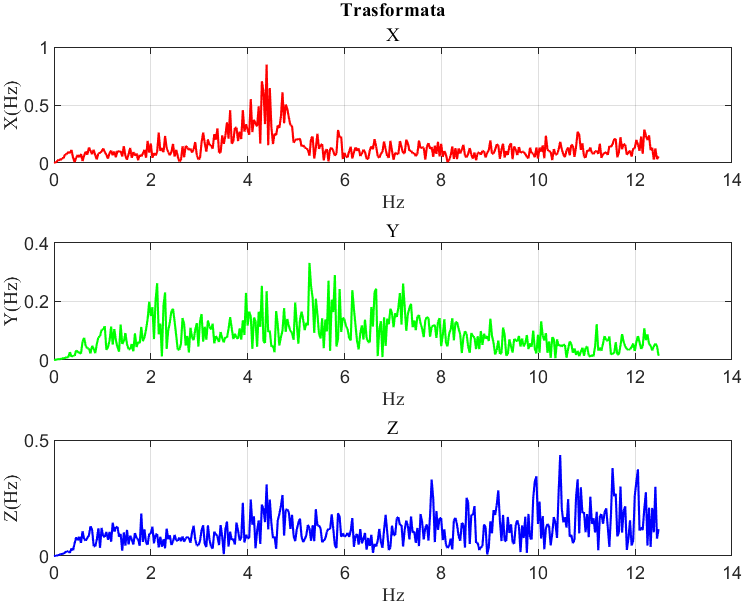
\includegraphics[height=.8\textheight]{figure/Acc/Trasformata/Trasformata}
	\end{frame}

	\begin{frame}{{Spettro}}
		\centering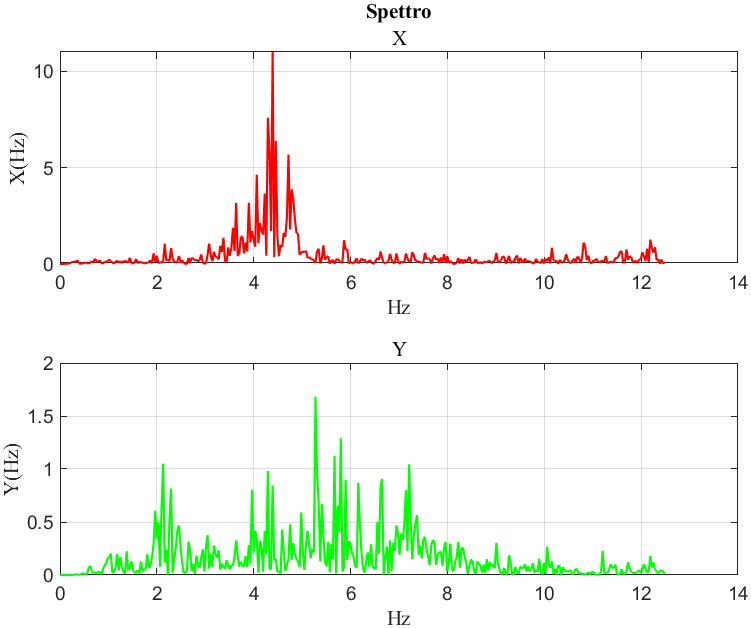
\includegraphics[height=.8\textheight]{figure/Acc/Trasformata/Spettro}
	\end{frame}
	
	\begin{frame}
		\color{blue}\centering\huge{\textbf{Trasformata Accelerazione}}
	\end{frame}
	
	\begin{frame}{{Trasformata Accelerazione 1}}
		\centering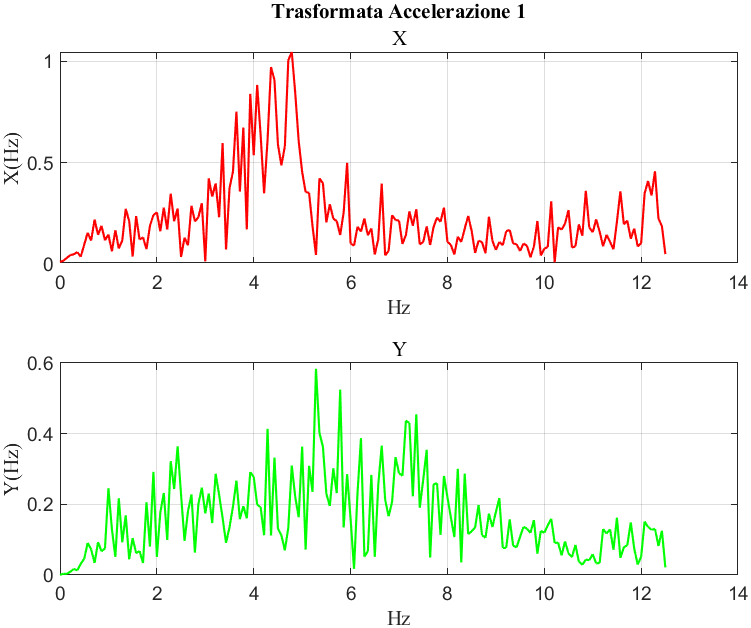
\includegraphics[height=.8\textheight]{figure/Acc/Trasformata/Trasformata Accelerazione 1}
	\end{frame}
	
	\begin{frame}{{Trasformata Idle 1}}
		\centering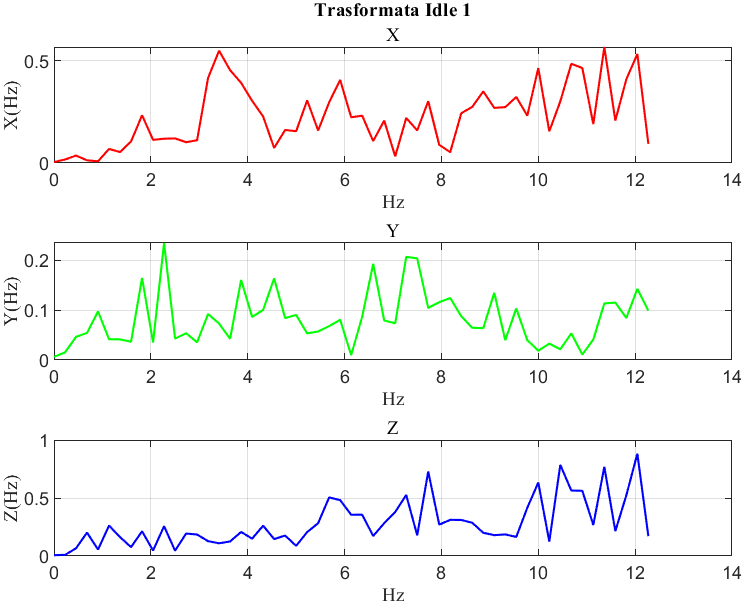
\includegraphics[height=.8\textheight]{figure/Acc/Trasformata/Trasformata Idle 1}
	\end{frame}
	
	\begin{frame}{{Trasformata Accelerazione 2}}
		\centering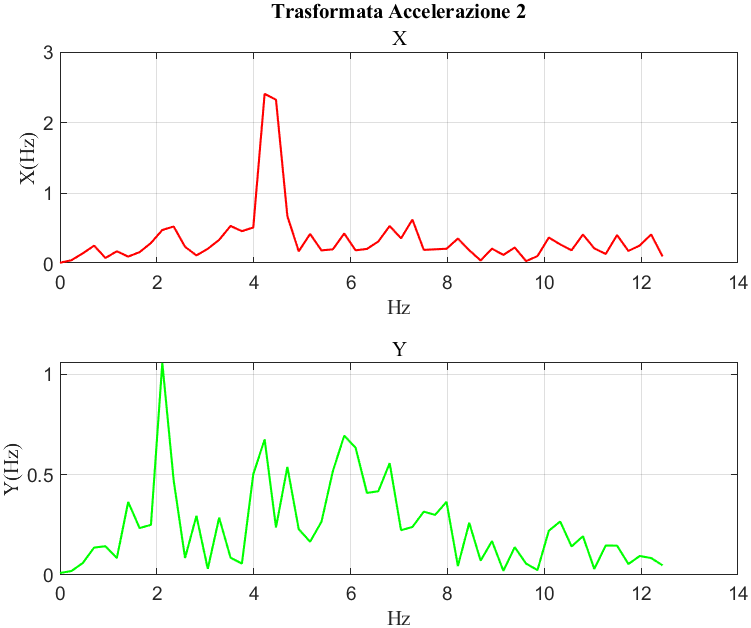
\includegraphics[height=.8\textheight]{figure/Acc/Trasformata/Trasformata Accelerazione 2}
	\end{frame}
	
	\begin{frame}{{Trasformata Idle 2}}
		\centering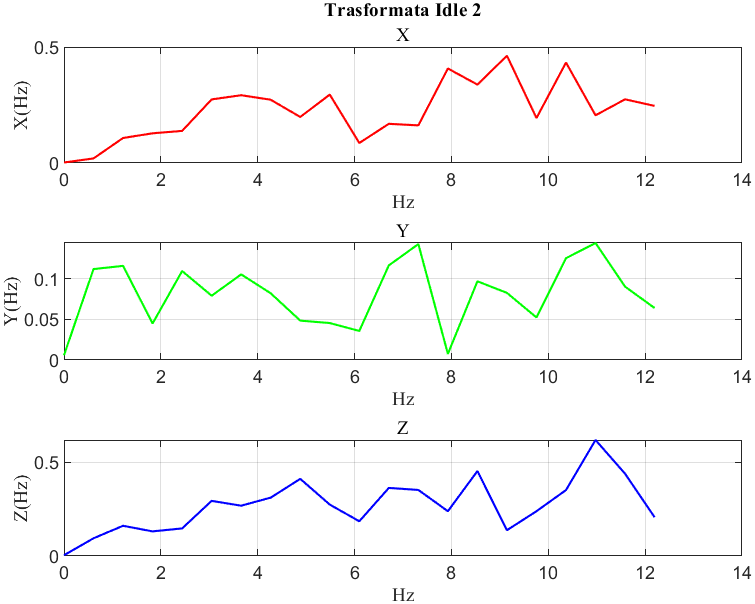
\includegraphics[height=.8\textheight]{figure/Acc/Trasformata/Trasformata Idle 2}
	\end{frame}
	
	\begin{frame}{{Trasformata Brake}}
		\centering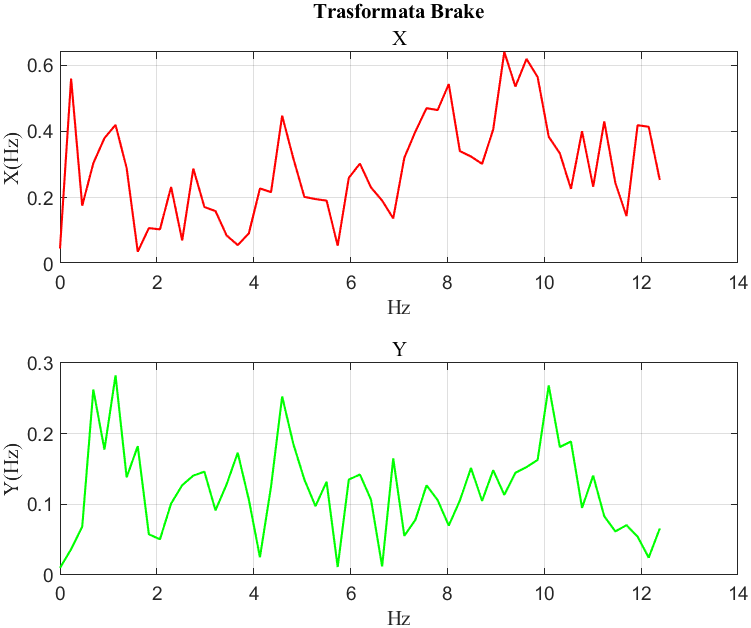
\includegraphics[height=.8\textheight]{figure/Acc/Trasformata/Trasformata Brake}
	\end{frame}
	
	\begin{frame}{{Ampiezza Media}}
		\begin{minipage}{.45\textwidth}
			\centering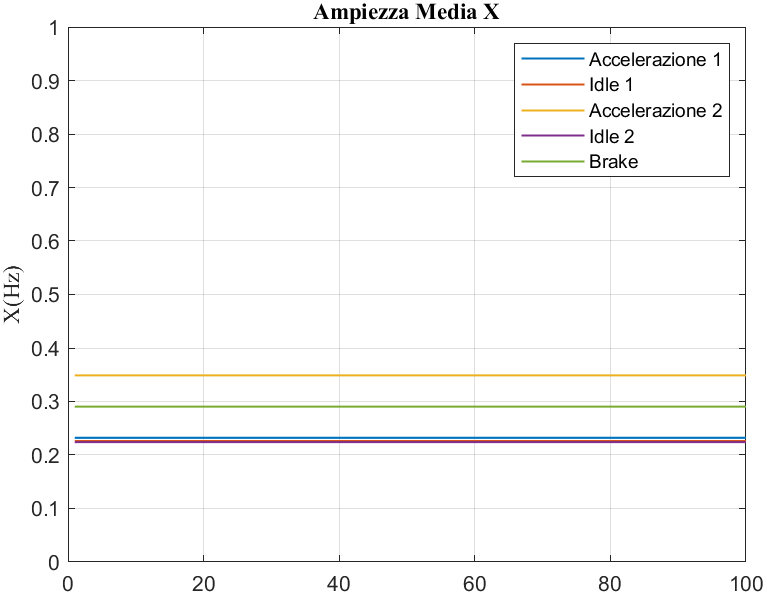
\includegraphics[width=.9\textwidth]{figure/Acc/Trasformata/Ampiezza MediaX}
		\end{minipage}
		\hspace{.05\textwidth}
		\begin{minipage}{.45\textwidth}
			\centering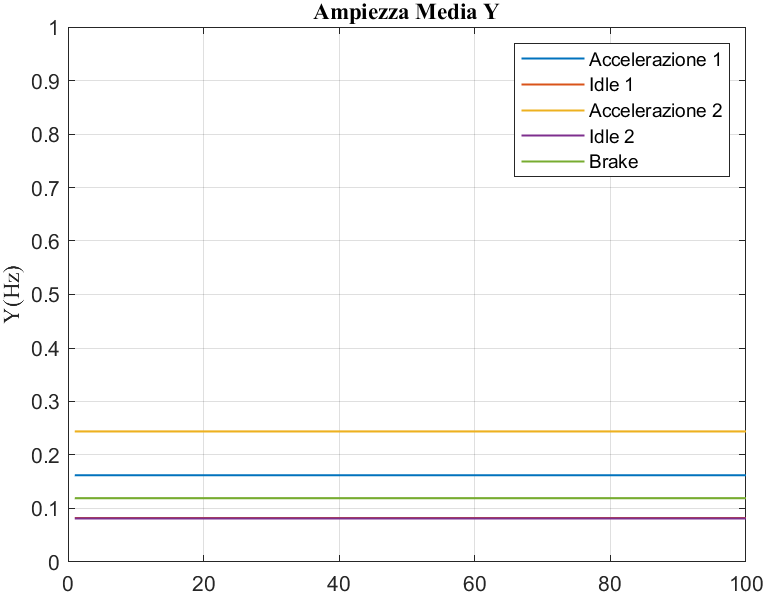
\includegraphics[width=.9\textwidth]{figure/Acc/Trasformata/Ampiezza MediaY}
		\end{minipage}
	\end{frame}

	\begin{frame}{{Frequency Centroid}}
		\begin{minipage}{.45\textwidth}
			\centering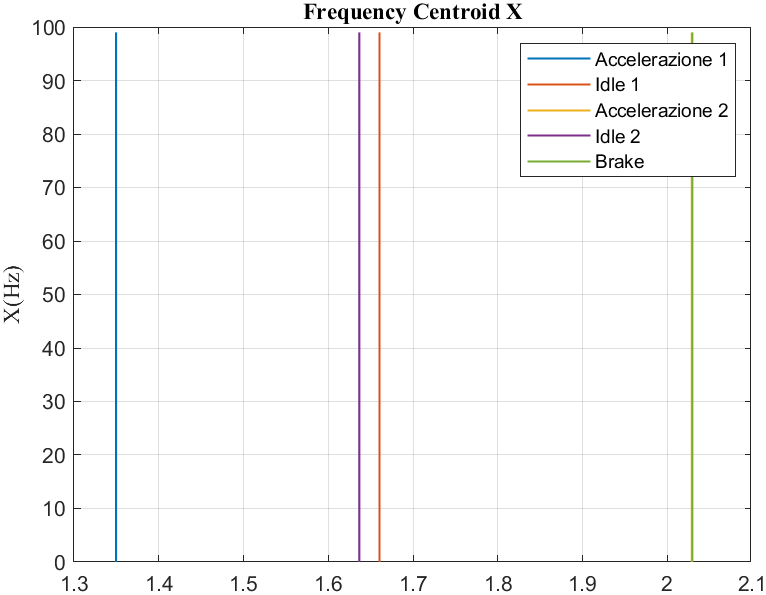
\includegraphics[width=.9\textwidth]{figure/Acc/Trasformata/Frequency CentroidX}
		\end{minipage}
		\hspace{.05\textwidth}
		\begin{minipage}{.45\textwidth}
			\centering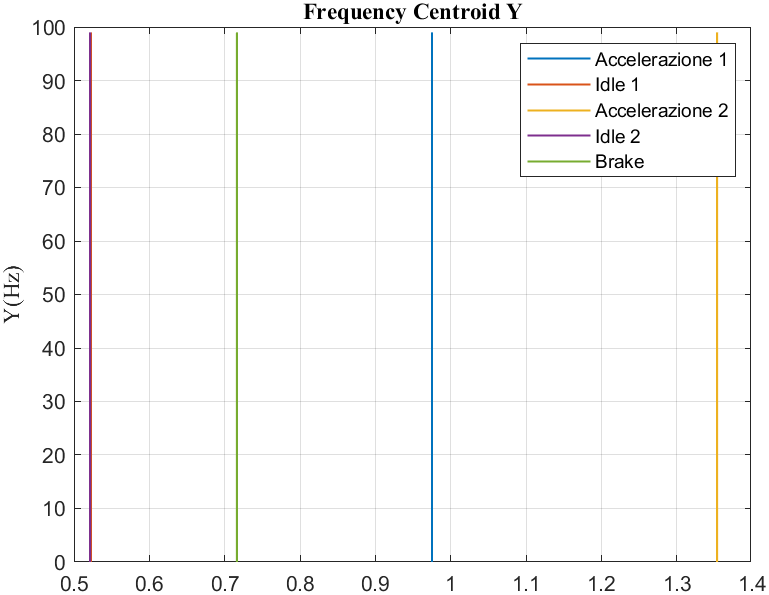
\includegraphics[width=.9\textwidth]{figure/Acc/Trasformata/Frequency CentroidY}
		\end{minipage}
	\end{frame}
	
	\begin{frame}{{Frequency Variance}}
		\begin{minipage}{.45\textwidth}
			\centering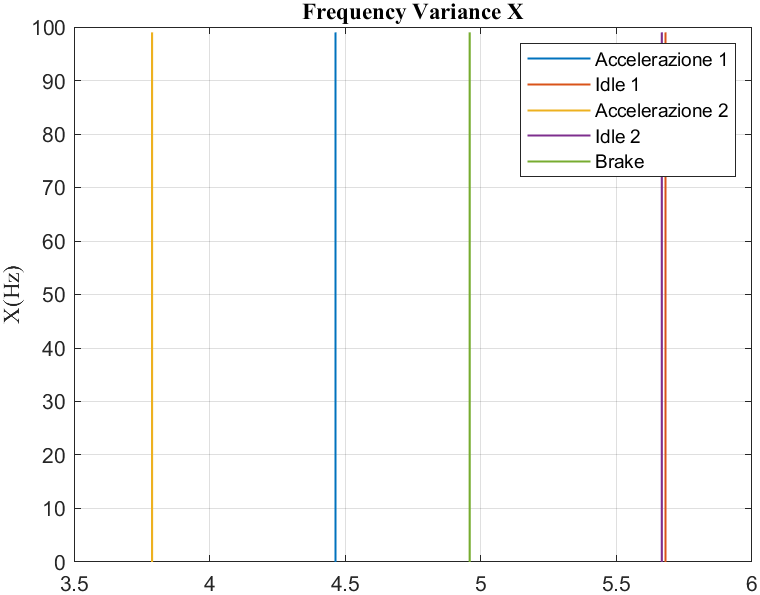
\includegraphics[width=.9\textwidth]{figure/Acc/Trasformata/Frequency VarianceX}
		\end{minipage}
		\hspace{.05\textwidth}
		\begin{minipage}{.45\textwidth}
			\centering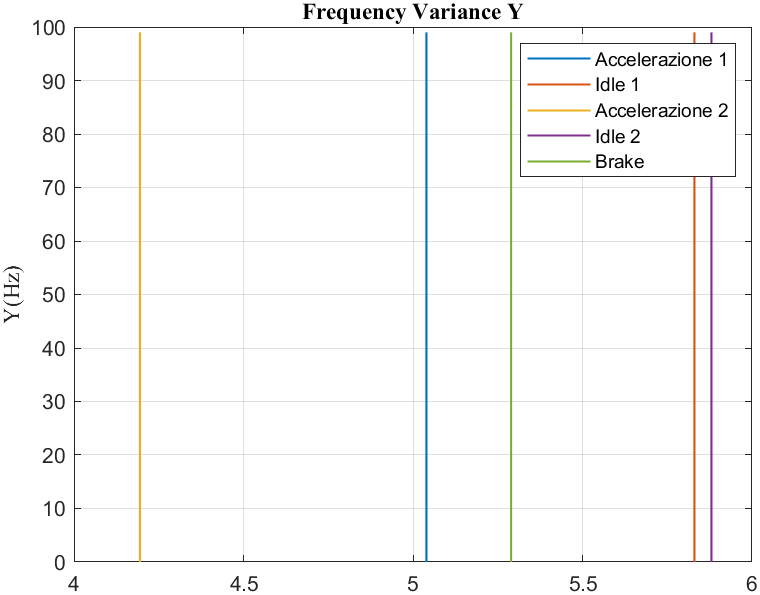
\includegraphics[width=.9\textwidth]{figure/Acc/Trasformata/Frequency VarianceY}
		\end{minipage}
	\end{frame}
	
	\begin{frame}
		\color{blue}\centering\huge{\textbf{Spettro Accelerazione}}
	\end{frame}
	
	\begin{frame}{{Spettro Accelerazione 1}}
		\centering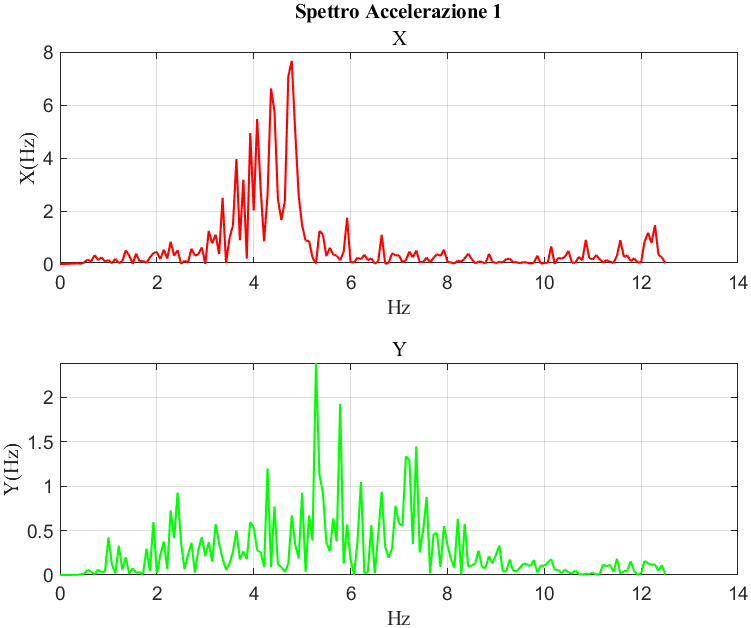
\includegraphics[height=.8\textheight]{figure/Acc/Trasformata/Spettro Accelerazione 1}
	\end{frame}
	
	\begin{frame}{{Spettro Idle 1}}
		\centering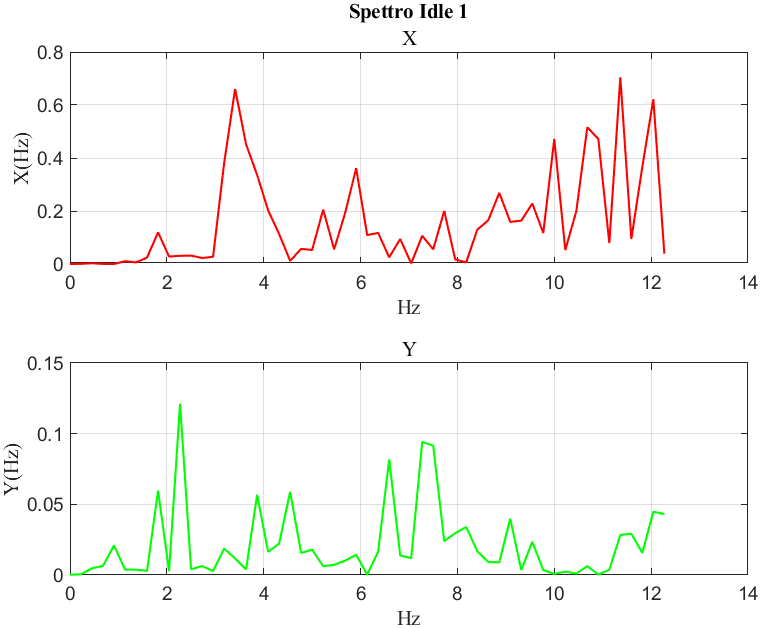
\includegraphics[height=.8\textheight]{figure/Acc/Trasformata/Spettro Idle 1}
	\end{frame}
	
	\begin{frame}{{Spettro Accelerazione 2}}
		\centering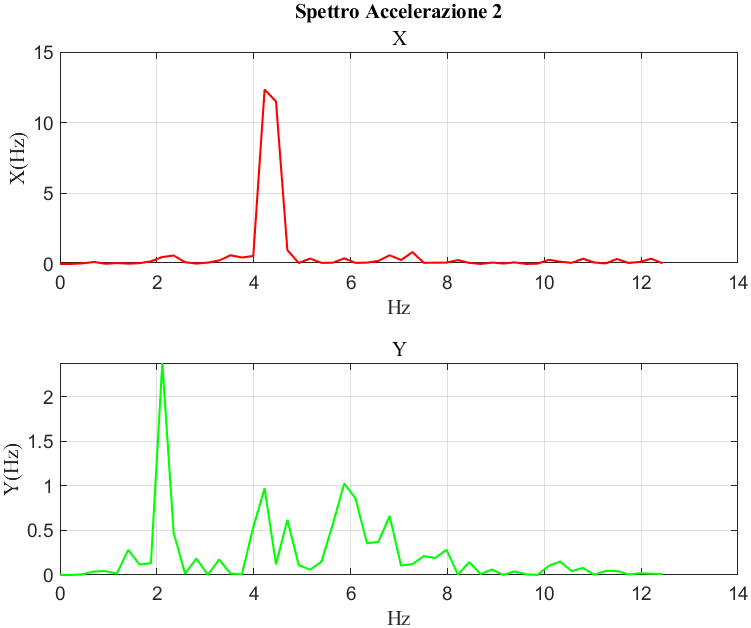
\includegraphics[height=.8\textheight]{figure/Acc/Trasformata/Spettro Accelerazione 2}
	\end{frame}
	
	\begin{frame}{{Spettro Idle 2}}
		\centering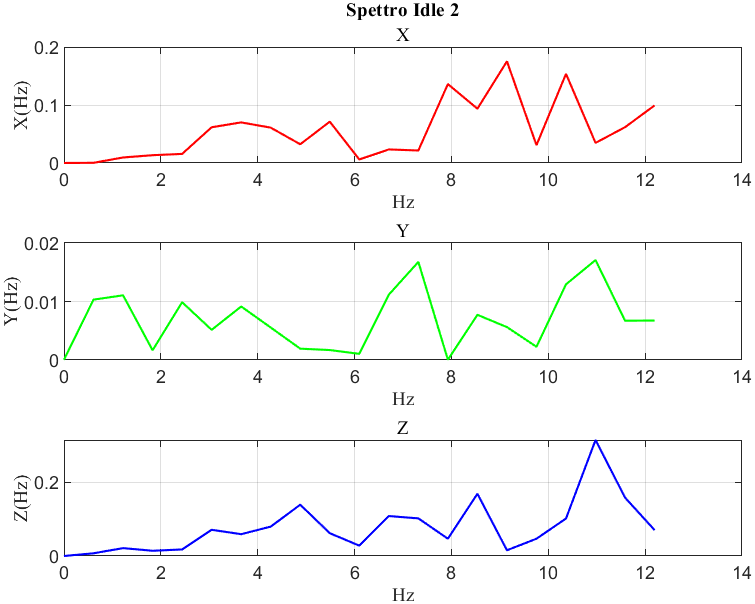
\includegraphics[height=.8\textheight]{figure/Acc/Trasformata/Spettro Idle 2}
	\end{frame}
	
	\begin{frame}{{Spettro Brake}}
		\centering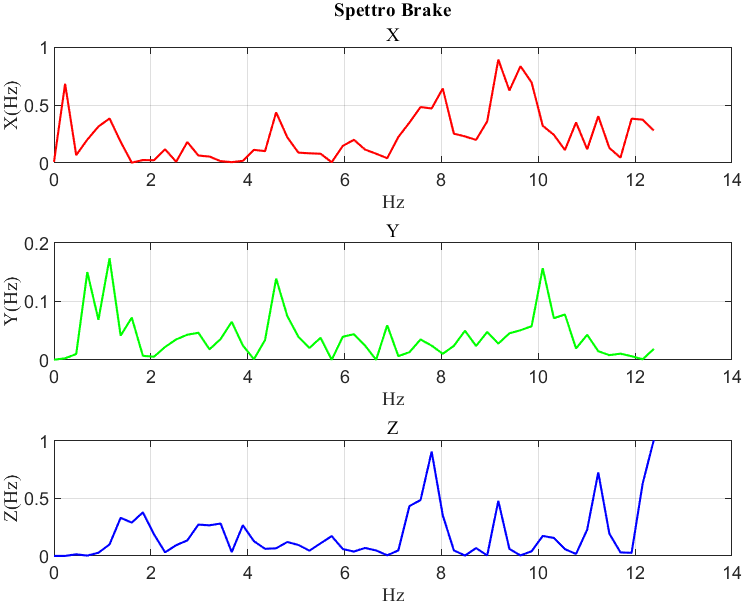
\includegraphics[height=.8\textheight]{figure/Acc/Trasformata/Spettro Brake}
	\end{frame}
	
	\begin{frame}{{Spectral EntropyX}}
		\begin{minipage}{.45\textwidth}
			\centering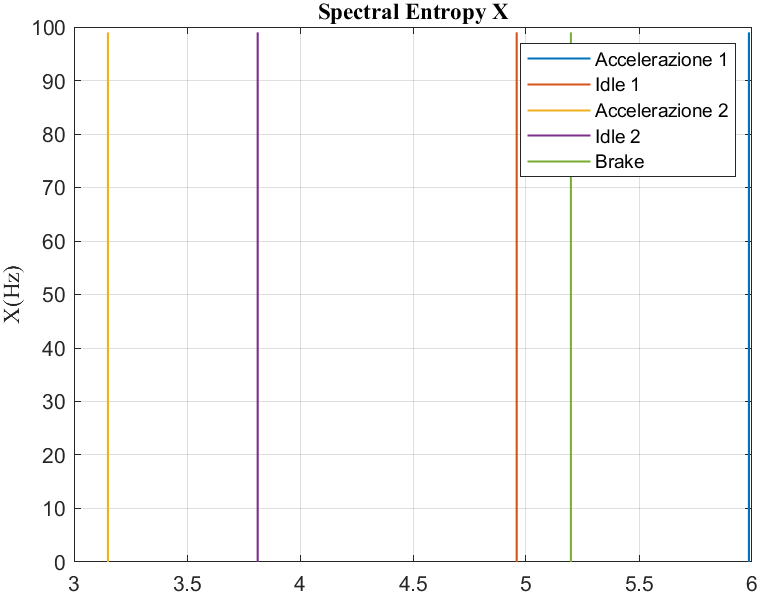
\includegraphics[width=.9\textwidth]{figure/Acc/Trasformata/Spectral EntropyX}
		\end{minipage}
		\hspace{.05\textwidth}
		\begin{minipage}{.45\textwidth}
			\centering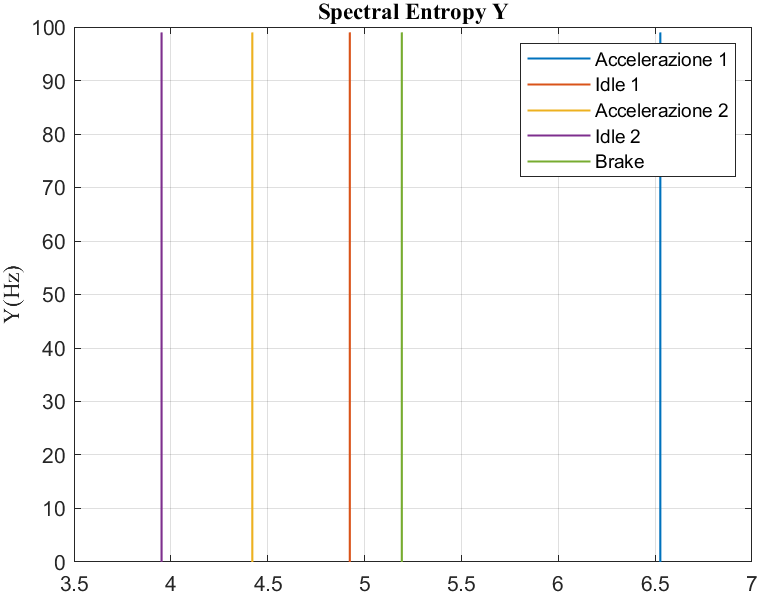
\includegraphics[width=.9\textwidth]{figure/Acc/Trasformata/Spectral EntropyY}
		\end{minipage}
	\end{frame}
	
\end{document}